\documentclass[10pt,a4paper]{article}

\usepackage[T1]{fontenc}
\usepackage[utf8]{inputenc}
\usepackage{mathpazo}
\usepackage{microtype}
\usepackage[a4paper,margin=1.6cm,top=1.5cm,bottom=1.7cm]{geometry}
\usepackage{graphicx}
\usepackage{booktabs}
\usepackage{tabularx}
\usepackage{array}
\usepackage{float}
\usepackage{flafter}
\usepackage[font=small,labelfont=bf,skip=3pt]{caption}
\usepackage{enumitem}
\usepackage{xcolor}
\usepackage{tikz}
\usetikzlibrary{arrows.meta,positioning}
\usepackage{titlesec}
\usepackage{xurl}
\usepackage[colorlinks=true,linkcolor=accent,urlcolor=accent]{hyperref}

\definecolor{accent}{HTML}{2A78D6}
\definecolor{quiet}{HTML}{52514E}
\definecolor{greyfill}{HTML}{EFEEEA}
\definecolor{bluefill}{HTML}{E3EEFB}

\setlist{nosep,leftmargin=1.3em}
\setlength{\parskip}{3pt}
\setlength{\parindent}{0pt}
\setlength{\textfloatsep}{6pt}
\setlength{\floatsep}{5pt}
\setlength{\intextsep}{5pt}
\emergencystretch=1.5em
\titleformat{\section}{\large\bfseries}{\thesection}{0.6em}{}
\titleformat{\subsection}{\normalsize\bfseries}{\thesubsection}{0.6em}{}
\titlespacing*{\section}{0pt}{8pt}{3pt}
\titlespacing*{\subsection}{0pt}{5pt}{1pt}
\newcolumntype{L}[1]{>{\raggedright\arraybackslash}p{#1}}
\newcommand{\q}[1]{\textit{``#1''}}

\begin{document}

\begin{center}
{\Large\bfseries RAG on the GDPR: Bi-Encoder Retrieval vs.\ Cross-Encoder Re-Ranking}\\[4pt]
Prakash Bhabad \quad$\cdot$\quad 19 October 2026\\[2pt]
{\small Code (notebook \texttt{rag\_assignment.ipynb}, results and outputs): \url{https://github.com/Pakkabhabad18/lma-rag-reranking-gdpr}}
\end{center}

%=====================================================================
\section*{Setup}

\textbf{Document.} I used the GDPR (Regulation (EU) 2016/679), the official 88-page PDF from EUR-Lex.
I chose it because it has two parts that use the same words: 173 \emph{recitals}, which explain the background and are not binding, and 99 \emph{articles}, which contain the actual rules.
Many articles also put a rule in one paragraph and its exceptions (\q{Paragraph 1 shall not apply if\ldots}) in another.
This makes it easy for retrieval to find a passage that is on the right topic but does not answer the question.

\textbf{Text and chunks.} I extracted the text with PyMuPDF.
Footnotes are printed in 8.5\,pt and body text in 9.6\,pt, so I removed footnotes by font size and the page headers by pattern.
(Removing footnotes by their text deleted the real recital 171, which starts with \q{Directive 95/46/EC}, so I switched to font size.)
I split the text at recital and article boundaries and cut anything longer than 200 words into 200-word windows with a 40-word overlap.
This gave \textbf{434 chunks} (214 from recitals, 220 from articles); 200 words is about 260 tokens, below the 512-token limit of both models.

\begin{figure}[H]
\centering
\begin{minipage}[c]{0.45\linewidth}
\footnotesize
\begin{tabular}{@{}L{1.95cm} L{5.6cm}@{}}
\toprule
Bi-encoder & \texttt{all-MiniLM-L6-v2} (384-dim, normalised) \\
Vector store & FAISS \texttt{IndexFlatIP}: exact search; inner product of normalised vectors = cosine \\
Cross-encoder & \texttt{ms-marco-MiniLM-L-6-v2} \\
LLM & Gemini (\texttt{3.7-flash}; K1, K3 on \texttt{3.5-flash}), temperature 0, thinking off \\
Prompt & identical for both; use only the passages, say what is missing, cite the article \\
Hardware & MacBook Air (Apple Silicon), CPU only \\
\bottomrule
\end{tabular}
\end{minipage}\hfill
\begin{minipage}[c]{0.53\linewidth}
\centering
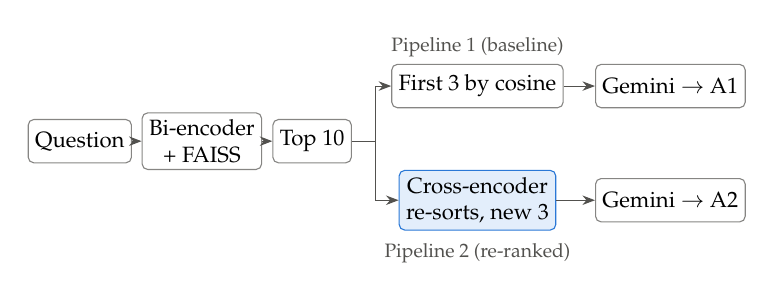
\begin{tikzpicture}[font=\footnotesize,
  box/.style={draw=quiet!70, rounded corners=2pt, minimum height=0.55cm, align=center, inner sep=2.5pt},
  blue/.style={box, draw=accent, fill=bluefill},
  arr/.style={-{Stealth[length=1.6mm]}, quiet}]
\node[box] (q) at (0,0) {Question};
\node[box] (bi) at (1.55,0) {Bi-encoder\\+ FAISS};
\node[box] (t) at (2.95,0) {Top 10};
\node[box] (p1) at (5.05,0.7) {First 3 by cosine};
\node[blue] (ce) at (5.05,-0.75) {Cross-encoder\\re-sorts, new 3};
\node[box] (a1) at (7.5,0.7) {Gemini $\to$ A1};
\node[box] (a2) at (7.5,-0.75) {Gemini $\to$ A2};
\draw[arr] (q) -- (bi); \draw[arr] (bi) -- (t);
\draw[quiet] (t.east) -- ++(0.3,0) coordinate (br);
\draw[arr] (br) |- (p1.west); \draw[arr] (br) |- (ce.west);
\draw[arr] (p1) -- (a1); \draw[arr] (ce) -- (a2);
\node[font=\scriptsize, text=quiet] at (5.05,1.2) {Pipeline 1 (baseline)};
\node[font=\scriptsize, text=quiet] at (5.05,-1.42) {Pipeline 2 (re-ranked)};
\end{tikzpicture}
\end{minipage}
\caption{Left: components. Right: both pipelines share the chunks, the top 10 and the prompt; only the choice of the 3 chunks given to Gemini differs, so any difference between Answer 1 and Answer 2 comes from that choice.}
\end{figure}

The Gemini free tier allows only a few requests per model per day, so my code moves to the next Flash model when one runs out.
Both answers for the same question always came from the same model, so the comparison stays fair.

%=====================================================================
\section{Architecture comparison: bi-encoder vs.\ cross-encoder}

\begin{figure}[H]
\centering
\begin{minipage}[c]{0.44\linewidth}
\centering
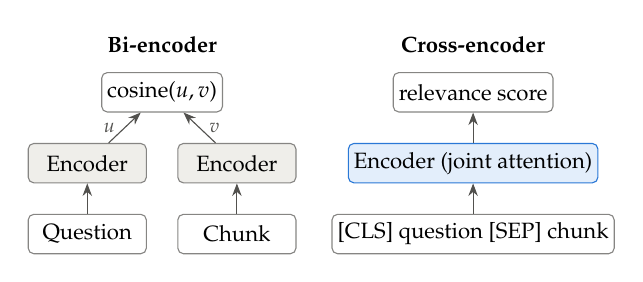
\begin{tikzpicture}[font=\footnotesize,
  box/.style={draw=quiet!70, rounded corners=2pt, minimum width=1.5cm, minimum height=0.5cm, align=center, inner sep=2pt},
  arr/.style={-{Stealth[length=1.6mm]}, quiet}]
\node[box] (q) at (0,0) {Question};
\node[box] (c) at (1.9,0) {Chunk};
\node[box, fill=greyfill] (e1) at (0,0.9) {Encoder};
\node[box, fill=greyfill] (e2) at (1.9,0.9) {Encoder};
\node[box] (s) at (0.95,1.8) {cosine($u,v$)};
\draw[arr] (q) -- (e1); \draw[arr] (c) -- (e2);
\draw[arr] (e1) -- node[left, font=\scriptsize] {$u$} (s);
\draw[arr] (e2) -- node[right, font=\scriptsize] {$v$} (s);
\node[font=\bfseries\footnotesize] at (0.95,2.4) {Bi-encoder};
\node[box, minimum width=3.0cm] (qc) at (4.9,0) {[CLS] question [SEP] chunk};
\node[box, minimum width=3.0cm, draw=accent, fill=bluefill] (e3) at (4.9,0.9) {Encoder (joint attention)};
\node[box] (r) at (4.9,1.8) {relevance score};
\draw[arr] (qc) -- (e3); \draw[arr] (e3) -- (r);
\node[font=\bfseries\footnotesize] at (4.9,2.4) {Cross-encoder};
\end{tikzpicture}
\end{minipage}\hfill
\begin{minipage}[c]{0.54\linewidth}
\footnotesize
\begin{tabular}{@{}L{1.75cm} L{3.1cm} L{3.1cm}@{}}
\toprule
 & Bi-encoder & Cross-encoder \\
\midrule
Input & question and chunk encoded separately & both in one sequence \\
Interaction & only at the end (cosine) & self-attention across all tokens \\
Precompute & yes, once & no \\
Work per question & 1 encoding + vector search & 1 encoding per candidate \\
Good at & right topic, fast, over everything & does it answer the question? \\
\bottomrule
\end{tabular}
\end{minipage}
\caption{The bi-encoder compresses each text into one vector before comparing; the cross-encoder compares token by token inside the model.}
\end{figure}

The main difference is \textbf{when the question and the chunk meet}.
\textbf{Bi-encoder:} each chunk goes through the model on its own and comes out as one 384-number vector (the mean of its token embeddings).
This is done once, before any question exists; at query time only the question is encoded, and the score is the cosine similarity of the two vectors.
Since the whole chunk is squeezed into one point, the vector says what the chunk is \emph{about}.
Short words that flip the meaning, such as \q{not}, \q{except} or \q{shall not apply}, carry little weight in that average.

\textbf{Cross-encoder:} the question and the chunk go in as one sequence.
Through self-attention, every question token can look at every chunk token in every layer, and the model outputs one score.
So it can check whether the chunk actually \emph{answers} the question, for example that \q{fired} in the question matches \q{dismissed} in the chunk.
The cost is that nothing can be computed in advance: each (question, chunk) pair needs its own full pass.

I saw this difference directly in the results: the bi-encoder often ranked a recital first, above the article that holds the rule (Recital 85 above Article 33, Recital 66 above Article 17, Recital 87 above Article 34).
Recitals are short, general summaries of one topic, so their single vector sits very close to the question's vector even when they do not contain the answer.

%=====================================================================
\section{Qualitative and rank shift analysis}

\subsection{How I tested}
I wrote 29 questions in four groups, phrased the way a normal person would ask them:
\textbf{keyword trap (K)}, everyday words where the regulation uses its own terms (\q{delete} vs.\ \q{erasure});
\textbf{exception (E)}, the general rule is in one chunk and the \q{except when} condition in another;
\textbf{negation (N)}, \q{not}, \q{cannot}, \q{without}, \q{no approval needed};
and \textbf{recital vs.\ article (D)}, a recital repeats the article's words without being the rule.
For each question I wrote down a \textbf{gold phrase}, a short exact phrase that only the answering passage contains (e.g.\ \q{shall not be dismissed or penalised}); the chunk containing it is the \emph{gold chunk}.
I recorded its rank in the bi-encoder's top 10 and after re-ranking. Only the top 3 reach Gemini, so each question gets one outcome.

\begin{figure}[H]
\centering
\begin{minipage}[c]{0.53\linewidth}
\footnotesize
\setlength{\tabcolsep}{3.5pt}
\begin{tabular}{@{}lcccccc@{}}
\toprule
Group & Both ok & Fixed & Hurt & Both miss & Not top 10 & Total \\
\midrule
Keyword trap & 1 & 1 & 1 & 1 & 1 & 5 \\
Exception & 1 & 1 & 0 & 0 & 3 & 5 \\
Negation & 7 & 2 & 0 & 0 & 5 & 14 \\
Recital vs.\ article & 4 & 0 & 0 & 0 & 1 & 5 \\
\midrule
\textbf{All} & \textbf{13} & \textbf{4} & \textbf{1} & \textbf{1} & \textbf{10} & \textbf{29} \\
\bottomrule
\end{tabular}
\end{minipage}\hfill
\begin{minipage}[c]{0.44\linewidth}
\centering
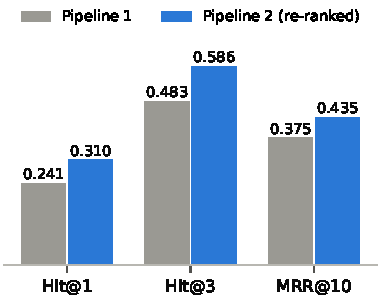
\includegraphics[width=0.94\linewidth]{figures/metrics.pdf}
\end{minipage}
\caption{Left: outcome per group (``fixed'' = gold chunk outside the top 3 before re-ranking and inside after; ``hurt'' = the reverse). Right: Hit@$n$ = share of questions with the gold chunk in the top $n$; MRR@10 = mean of 1/rank (0 if not in the top 10).}
\end{figure}

Re-ranking improves every measure.
Hit@3 matters most, because it is the share of questions where Gemini actually gets the right passage: 0.483 $\to$ 0.586, three more questions out of 29.
Hit@1 goes from 0.241 to 0.310, so the cross-encoder is also better at deciding which candidate is \emph{the} answer.
The gains are modest because 10 questions never had the gold chunk in the top 10 (Section~\ref{sec:limits}).

\subsection{Rank shifts}

\begin{figure}[H]
\centering
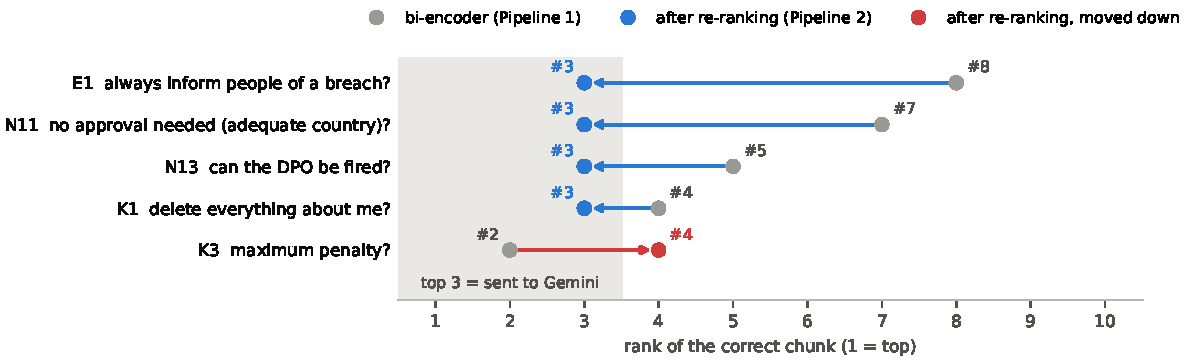
\includegraphics[width=0.8\linewidth]{figures/rank_shift.pdf}\\[3pt]
\footnotesize
\begin{tabular}{@{}l c l l l@{}}
\toprule
ID & Rank (P1 $\to$ P2) & Gold chunk & Pipeline 1 context (top 3) & Pipeline 2 context (top 3) \\
\midrule
E1 & 8 $\to$ 3 & Art.\ 34(3) & Rec.\ 87, Art.\ 33, Rec.\ 88 & Rec.\ 87, Rec.\ 85, \textbf{Art.\ 34} \\
N11 & 7 $\to$ 3 & Art.\ 45(1) & Rec.\ 107, Rec.\ 102, Rec.\ 103 & Rec.\ 107, Rec.\ 103, \textbf{Art.\ 45} \\
N13 & 5 $\to$ 3 & Art.\ 38(3) & Art.\ 38 (other chunk), Art.\ 37, Rec.\ 97 & Rec.\ 97, Art.\ 38, \textbf{Art.\ 38(3)} \\
K1 & 4 $\to$ 3 & Art.\ 17(1) & Rec.\ 66, Art.\ 33, Rec.\ 26 & Rec.\ 65, Rec.\ 66, \textbf{Art.\ 17} \\
K3 & 2 $\to$ 4 & Art.\ 83 & Art.\ 84, \textbf{Art.\ 83}, Rec.\ 148 & Rec.\ 149, Rec.\ 148, Rec.\ 150 \\
\bottomrule
\end{tabular}
\caption{Rank of the gold chunk before (grey) and after (colour) re-ranking for the five questions where the top 3 changed, and the 3 chunks each pipeline gave to Gemini (gold chunk in bold).}
\end{figure}

\subsection{Answer 1 vs.\ Answer 2}

\textbf{E1, exception (\#8 $\to$ \#3).} \q{Does a company always have to inform affected people about a data breach?}
Article 34(1) says people must be told when a breach is high-risk, and Article 34(3) lists when this is \emph{not} required.
The bi-encoder ranked that chunk 8th and filled the top 3 with Recital 87, Article 33 (notifying the \emph{authority}, not the people) and Recital 88.
Answer 1: \q{there is not enough information to fully answer whether a company always has to inform affected people}.
Answer 2: \q{No, a company does not always have to inform affected people}, followed by the three Article 34(3) cases (data made unintelligible e.g.\ by encryption, later measures removing the high risk, disproportionate effort).
The baseline \textbf{left out the essential exception}, and the question was about exactly that exception.

\textbf{K1, keyword trap (\#4 $\to$ \#3).} \q{Can I make a company delete everything it knows about me?}
The question says \q{delete}, the regulation says \q{erasure}. The bi-encoder's rank 2 was Article 33 on breach notification, which shares only general words such as \q{controller} and \q{personal data}.
Answer 1 worked only from Recital 66 and said the full conditions were missing; Answer 2 listed the six grounds of Article 17(1) and concluded that erasure is not unconditional.

\textbf{N11, negation (\#7 $\to$ \#3).} \q{Is no special approval needed to transfer data to a country the Commission considers adequate?}
Both answers said yes, but Answer 1 took this only from Recital 103, which is not binding, while Answer 2 cited Article 45(1), \q{shall not require any specific authorisation}.
Re-ranking did not change the conclusion here; it changed the \textbf{source} to the actual rule.

\textbf{N13, negation and synonym (\#5 $\to$ \#3).} \q{Can the data protection officer be fired for doing their job?}
\q{Fired} in the question, \q{dismissed or penalised} in the text. Article 38 was already ranked 1st by the bi-encoder, but it was the \emph{other} chunk of Article 38, without the dismissal rule (my chunking had split the article).
Answer 1: \q{there is not enough information to answer whether a data protection officer can be fired}. Answer 2: \q{No}, quoting Article 38(3).

\textbf{K3, the case where re-ranking made it worse (\#2 $\to$ \#4).} \q{What is the maximum penalty a company can get?}
The bi-encoder had Article 83 at rank 2, and Answer 1 was correct: up to EUR 10 million or 2\% of worldwide turnover under 83(4), and EUR 20 million or 4\% under 83(5).
The cross-encoder moved Recitals 149, 148 and 150 to the top because they talk about \q{penalties} in general, and Answer 2 said the maximum is not specified.
It was trained on web search queries (MS MARCO) and rewarded passages that \emph{discuss} penalties over the one that \emph{states} the number; Article 84 is even titled \q{Penalties} but covers national penalties.
So the cross-encoder is not always right.

\textbf{Did the baseline hallucinate?} No. When the right chunk was missing, Answer 1 either said the passages were not enough (E1, K1, N13) or answered from a recital instead of the article (N11).
I think this is because the prompt says to use only the given passages and to say what is missing.
Without that line the model would probably fill the gap from what it already knows about the GDPR, and the retrieval failure would be hidden behind a confident answer.
So in this setup a retrieval miss shows up as an \textbf{omission}, not a hallucination.

\subsection{When re-ranking cannot help}
\label{sec:limits}

\noindent
\begin{minipage}[t]{0.53\linewidth}
\vspace{0pt}
For 10 of the 29 questions the gold chunk was not in the bi-encoder's top 10, so the cross-encoder never saw it.
To check whether the cross-encoder would have found it, I let both models rank all 434 chunks for these questions (Figure~\ref{fig:full}).
For three questions (K2, N4, E2) the cross-encoder would have put the gold chunk in its top 4, so a larger candidate list would have fixed them.
For others (E3, N7, N8, N12) both models rank it far down, so the problem there is the models themselves, not only the first stage.
Most of these use plain words for a legal concept: \q{subcontractor} for \q{another processor}, \q{computer program} for \q{automated processing}.
\end{minipage}\hfill
\begin{minipage}[t]{0.43\linewidth}
\vspace{0pt}
\centering
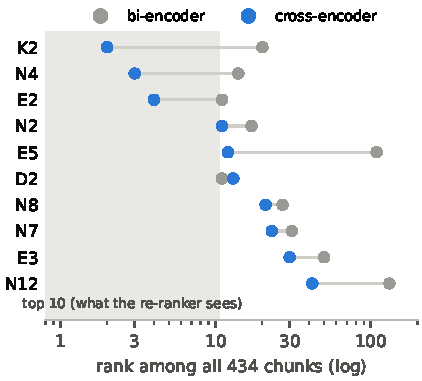
\includegraphics[width=0.95\linewidth]{figures/full_ranks.pdf}
\captionof{figure}{Rank of the gold chunk among all 434 chunks for the 10 questions where it missed the top 10.}
\label{fig:full}
\end{minipage}

%=====================================================================
\section{Latency profiling}

I timed each step separately with \texttt{time.perf\_counter()}, after three warm-up questions, over 29 questions $\times$ 10 repeats = 290 runs on the CPU.

\begin{figure}[H]
\centering
\begin{minipage}[c]{0.49\linewidth}
\footnotesize
\begin{tabular}{@{}lrrr@{}}
\toprule
Retrieval step (ms per question) & Mean & Median & p95 \\
\midrule
Query embedding (bi-encoder) & 11.67 & 10.91 & 15.74 \\
FAISS search, 434 chunks & 0.05 & 0.04 & 0.06 \\
Cross-encoder, 10 pairs + sort & 163.69 & 157.88 & 205.44 \\
\midrule
\textbf{Pipeline 1 retrieval} & 11.72 & 10.95 & 15.87 \\
\textbf{Pipeline 2 retrieval} & 175.41 & 168.99 & 220.91 \\
\midrule
\multicolumn{4}{@{}l}{\textit{End to end (median retrieval + median Gemini call, \texttt{3.8-flash}):}} \\
Pipeline 1: 11 + 4{,}516 & & \multicolumn{2}{r}{= 4{,}527} \\
Pipeline 2: 169 + 4{,}248 & & \multicolumn{2}{r}{= 4{,}417 (re-rank 3.6\%)} \\
\bottomrule
\end{tabular}
\end{minipage}\hfill
\begin{minipage}[c]{0.47\linewidth}
\centering
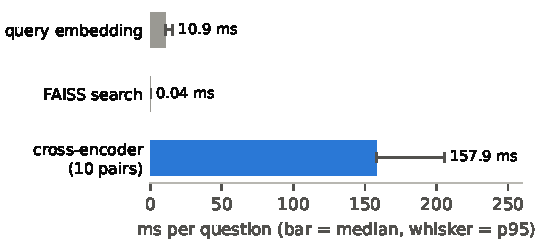
\includegraphics[width=\linewidth]{figures/latency.pdf}
\end{minipage}
\caption{Retrieval time per question. The FAISS search is almost free; the cross-encoder is the expensive step.}
\end{figure}

Re-ranking makes retrieval about \textbf{15 times slower} (11\,ms $\to$ 169\,ms); almost all of Pipeline 1's time is encoding the question, and the search over 434 vectors takes 0.04\,ms.
Next to a Gemini call of about 4.2--4.5 seconds, though, the extra 158\,ms is under 4\% of the total.
The Gemini time also changes a lot from call to call (3.1\,s to 6.0\,s across my runs), which is why Pipeline 2's total here is even slightly lower than Pipeline 1's; that is network noise, not a property of the pipelines.
Building the index (encoding all 434 chunks) took 4.7\,s once.

%=====================================================================
\section{Scaling: why not run the cross-encoder on everything?}

Because a cross-encoder cannot prepare anything ahead of time.
Its score comes from reading the question and the chunk \emph{together}, so for every new question it must run the full model once for every chunk in the collection.
A bi-encoder encodes the chunks once, offline; for a new question it encodes only the question and does one dot product per stored vector.

I measured this directly: the cross-encoder on all 434 chunks took \textbf{4.7\,s for a single question} (10.9\,ms per pair), already slower than the Gemini call, for just one document.
For larger collections I used that per-pair time, and for FAISS I measured a flat search over 100{,}000 random vectors (3.3\,ms).

\begin{figure}[H]
\centering
\begin{minipage}[c]{0.5\linewidth}
\centering
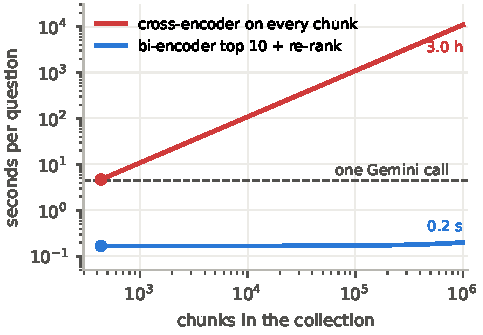
\includegraphics[width=0.95\linewidth]{figures/scaling.pdf}
\end{minipage}\hfill
\begin{minipage}[c]{0.46\linewidth}
\footnotesize
\begin{tabular}{@{}rrr@{}}
\toprule
Chunks & Cross-encoder on all & Top 10 + re-rank \\
\midrule
434 (measured) & 4.7 s & 0.17 s \\
10{,}000 & 1.8 min & 0.17 s \\
100{,}000 & 18 min & 0.17 s \\
1{,}000{,}000 & 3.0 h & 0.2 s \\
\bottomrule
\end{tabular}
\end{minipage}
\caption{Time per question as the collection grows (log scales). Points at 434 chunks are measured; the rest are estimates from the measured cost per pair and per vector.}
\end{figure}

A full cross-encoder ranking grows linearly with the collection, while retrieve-then-re-rank stays almost flat because the re-ranker always sees only 10 chunks.
With an approximate index (HNSW or IVF) instead of my exact flat index, the bi-encoder search would grow even more slowly.
So the sensible design is the one I built: the cheap bi-encoder for \emph{recall} over everything, then the expensive cross-encoder for \emph{precision} on a short list.
The trade-off is the size of that list, $k$: a larger $k$ would have rescued K2, N4 and E2, but re-ranking time grows linearly with $k$ (about 16\,ms per extra chunk here).

%=====================================================================
\section{Conclusion and limitations}

\begin{itemize}
\item Re-ranking helped where the bi-encoder's single vector loses detail: an exception kept in a different chunk (E1), negated questions (N11, N13) and everyday words for legal terms (K1, N13). In all four wins the gold chunk sat at ranks 4--8 and moved up to rank 3.
\item It is not free of errors: in K3 it preferred general recitals over the article with the actual number.
\item On this document the bi-encoder's main weakness was preferring recitals, which summarise a topic, over articles, which state the rule.
\item The bigger limit is recall: 10 of 29 gold chunks never reached the re-ranker. A larger $k$, or better chunking for long articles, would matter more than a stronger re-ranker.
\item Re-ranking costs little in practice (about 160\,ms, under 4\% of end-to-end), while scoring the whole collection with a cross-encoder is not usable beyond a few hundred chunks.
\end{itemize}

\textbf{Limitations.} One document and 29 questions that I wrote myself, so the numbers are indicative, not general.
Both encoders are small MiniLM models.
Because of free-tier limits, the answers came from more than one Gemini Flash version, although both answers of each question always used the same one.
Gemini latency includes network time and varies between runs.

\end{document}
